\subsection{Moving a Cube}
Before moving a cube, the cube must first be rotated to a different face.
This rotation is entirely based on whether the die rolled was even or odd.
After the cube has been rotated, it is then moved the indicated number of spaces orthogonally in any direction on the board, though never crossing back over the starting line.

It is important to note the following restrictions:
\begin{itemize}
    \item Cubes cannot move diagonally.
    \item Cubes cannot pass over each other.
    \item A cube can only be moved once in a turn.
    \item Cubes cannot enter the same square more than once on a turn.
    \item Once a cube leaves the Bank, it cannot re-enter unless as part of a stack (See \textit{Bearing Off} Section~\ref{sec:bearing-off}).
    \item Cubes in the Bank must finish their move on the Grid, if able.
    \item A cube cannot form a Set (Section~\ref{sec:bearing-off}) or Pinch (Section~\ref{sec:pinching}) on the same turn it left the Bank.
\end{itemize}

\paragraph{If the Die Shows Even} The cube's face value is increased to the next available value
$$1 \to 8 \to 16 \to 24 \to 32 \to 40 \to 1$$
\paragraph{If the Die Shows Odd} The cube's face value is decreased to the previous value
$$40 \to 32 \to 24 \to 16 \to 8 \to 1 \to 40$$

\note In either case, a roll-over happens if a player tries to increase or decrease past the highest or lowest value respectively.

\begin{figure}[!ht]
    \centering
    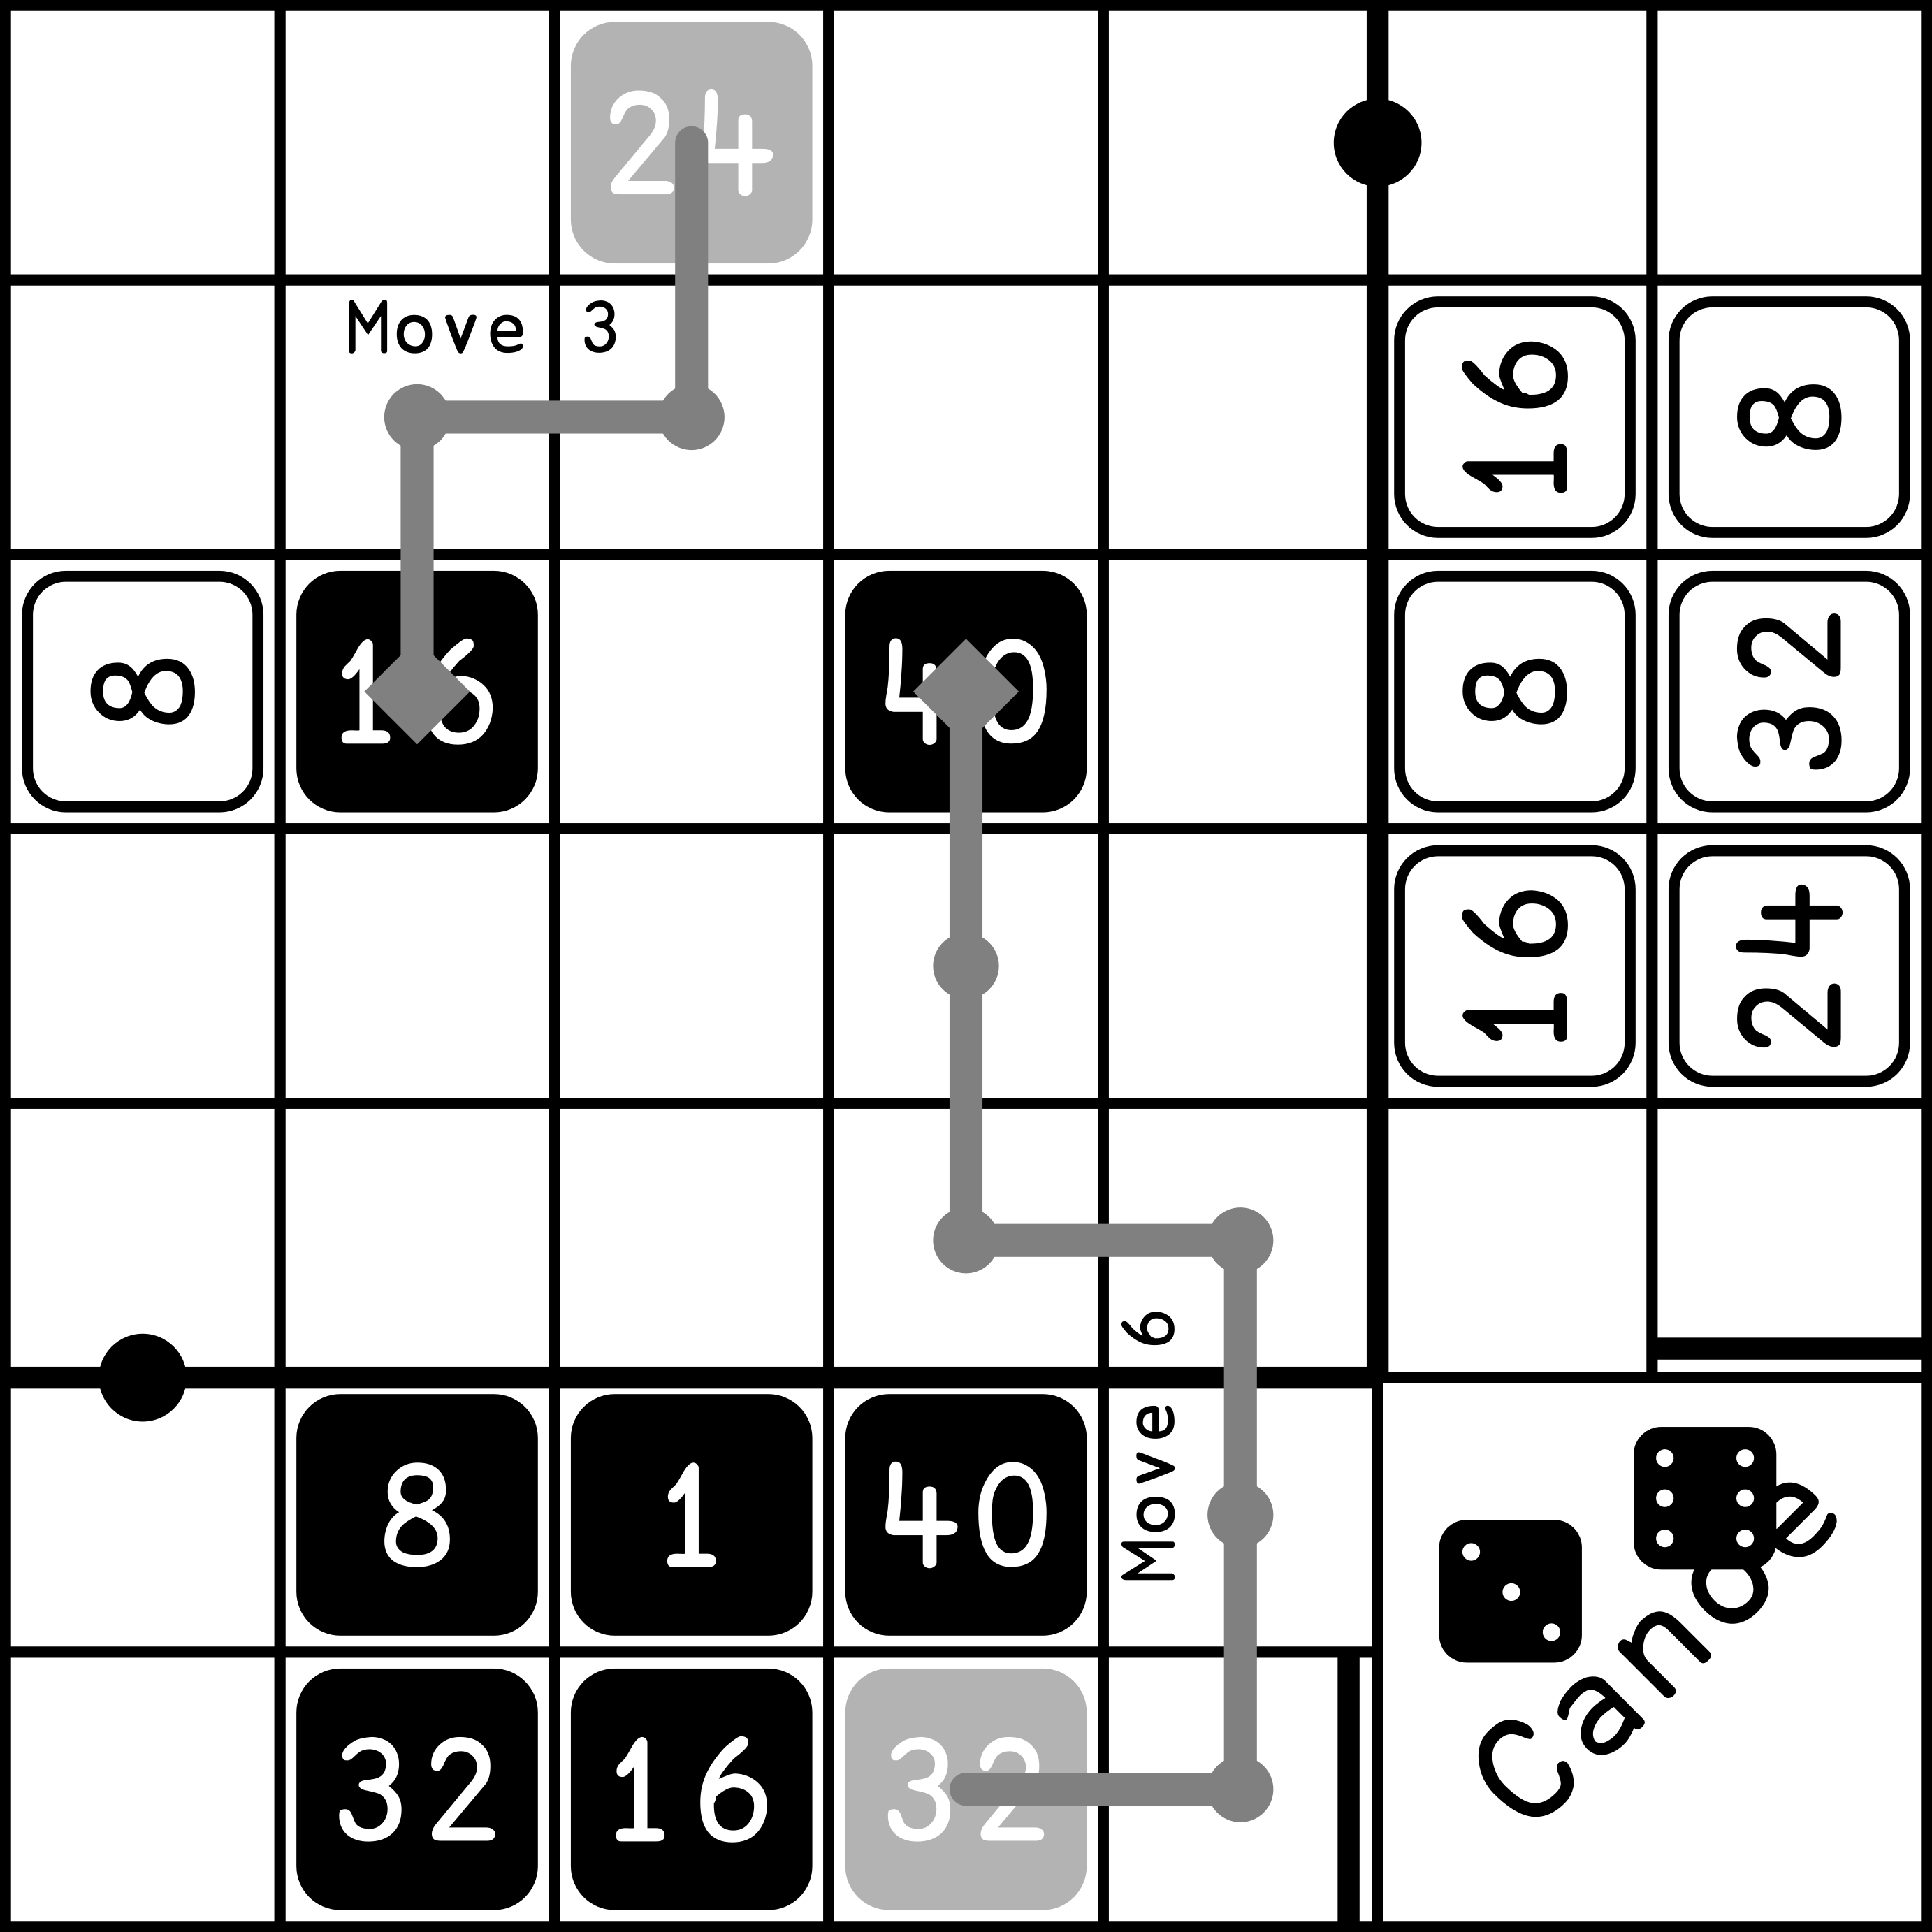
\includegraphics[width=8cm]{../graphics/movement}
    \caption{Example Move}
    \label{fig:move}
\end{figure}

\example In Figure~\ref{fig:move}, Billy rolled a \epsdice{6} and a \epsdice{3}, and has decided to move his 24 cube three spaces. 
He first rotates the cube so it shows 16 before moving it those three spaces. 
Next he wants to move his 32 cube six spaces, he first rotates the cube so it instead shows 40, and then moves it six spaces.

\subsubsection{Stymie}
In the event that a player has exactly two cubes left, and both share the same number and are either adjacent or have an even number of spaces between them, then that player may choose to call ``Stymie'' and only roll one die on their turn.